% !TeX root = ../SDonchezThesis.tex

\chapter{Related Work}\label{ch:relatedWork}
Although the introduction of FPGAs into a cloud based environment has been a recent development, there exists some body of research conducted on such systems, as well as their security. A brief survey of those efforts is provided below, culminating in a detailed analysis of the specific prior work which proposes the architecture this effort seeks to extend.

\section{FPGAs in a Cloud Environment}\label{sec:fpgaCloud}
In \cite{chen_enabling_2014}, researchers from IBM and Microsoft, among other institutions, propose a robust architecture for the implementation of cloud based FPGAs utilizing the Openstack framework. In their design, ``Compute Nodes'' (heterogenous systems) are subdivided into a number of Virtual Machines, each containing a Virtual FPGA comprising a portion of the physical FPGA. This design is captured in Figure \ref{fig:chen_enabling_architecture}, below.

\begin{figure}
    \centering
    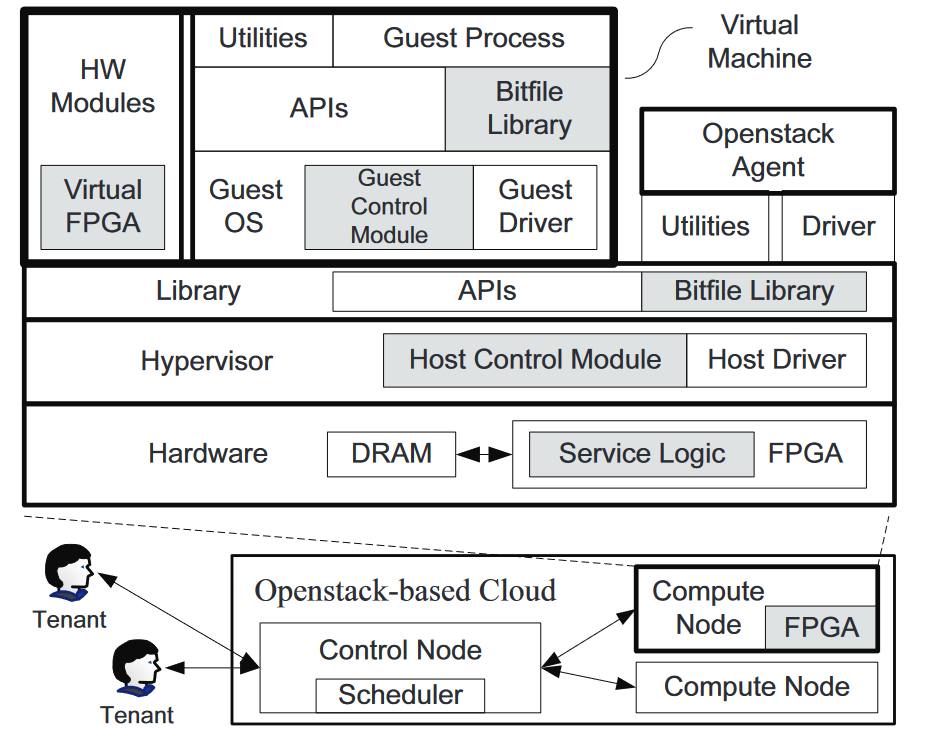
\includegraphics{chen_enabling_architecture.png}
    \caption[Cloud FPGA Architecture]{Cloud FPGA Architecture. Image courtesy of ~\cite{chen_enabling_2014}.}
    \label{fig:chen_enabling_architecture}
\end{figure}


\section{Cloud FPGA Security}\label{sec:cloudFPGASecurity}
Two recent works, \cite{jin_security_2020} and \cite{turan_trust_2020} have conducted comprehensive surveys of the state security in cloud based FPGAs. In \cite{jin_security_2020}, the authors discuss several avenues by which multi-tenant FPGAs present new vulnerabilities for FPGA compromise. Additionally, they present a number of solutions for access control in a multi-tenant environment. One such suggestion is the inclusion of a Secure Authentication Module (SAM), which enables verification of each IP by means of a challenge-response protocol. The work does not go into detail about this implementation, but one potential for SAM implementation is Xilinx and Silex Insight's Hardware Security Module (HSM), which facilitates secure key storage and management, as well as a cryptographic engine that could be harnessed for the secure key storage.

The authors of \cite{jin_security_2020} also discuss efforts investigating a novel method of mitigating the other primary concern of a co-tenant FPGA: side channel attacks. As the presence of malicious tenants fully under their own control (as opposed to reliant on an obscured trigger) poses a much higher threat, additional safeguards are needed to limit the amount of information that can be gained from the traditional side channels. One key vulnerability they focus on is power draw. To mitigate the extraction of data through the power side channel, they discuss research that proposes actively injecting noise into power traces, as well as attempting to actively adjust power draw to produce a constant consumption rate regardless of the needs of the functional logic.

The authors of \cite{turan_trust_2020} similarly surveys a wide body of research in the area of cloud computing. One particularly noteworthy idea they present is a research effort that attempts to provide authenticity to a bitstream by associating it with an accompanying software application, which runs on the CPU. In this model, the secure software is responsible for decrypting and programming the bitstream, providing the opportunity for suppliers to ensure that the bitstream is not compromised.

Similar to the efforts discussed previously in this section, \cite{turan_trust_2020} also presents an effort to facilitate the secure implementation of Multi-Tenant FPGAs. Specifically, they discuss an effort wherein a specific FPGA can be provided from a trusted vendor with a pair of asymmetric keys pre-configured, such that the integrator can provide the public key to IP providers to encrypt their bitstreams. In this way, no substantial storage overhead or complex key negotiation effort is required at the time of reconfiguration.

\section{Multi-Tenant Cloud Based FPGA Implementation in Literature}\label{sec:LitImpl}
In "Cryptographically Secure Multi-Tenant Provisioning of FPGAs"\cite{bag_cryptographically_2020} Bag et al. outline a comprehensive architecture for the implementation of a cloud-compatible FPGA architecture, from which much of the work undertaken by this research effort is derived. This work proposes a platform wherein multiple discrete tenants can occupy "Virtual FPGA" (VFPGA) partitions of a larger Physical FPGA (PFPGA) device in a secured environment. In their proposal, they utilize Key Aggregation Cryptography (KAC) to facilitate the encryption of a symmetric (AES) key, which in turn can be used to decrypt tenant bitstreams within their allocated partition. In this implementation, they utilize a single KAC decryption engine at the PFPGA level, which extracts the AES key and furnishes it to individual AES engines at the VFPGA level. The authors claim that by implementing their design in this manner, the only party which the tenant is required to trust is the FPGA Vendor, who provides the public and private keys used by the KAC engine to decrypt the symmetric key.

\subsection{Implementation Evaluation}\label{subsec:LitEval}
However, this claim is not completely true. By virtue of decrypting the symmetric key at the PFPGA layer, the Cloud Service Provider (CSP) is in possession of both the encrypted bitstream and the symmetric key required to decrypt it. In essence, this is equivalent to them having access to the IP contained within the bitstream itself. Therefore, the tenant must necessarily also trust the CSP, which is not a policy compatible with the security needs of many would-be tenants.Furthermore, the decrypted AES key is stored into memory, which must be isolated. Unfortunately, resolving this concern by isolating this data from the greater PL is not feasible, as there can be only one entry point into the PL from the DDR, which must be shared with all users. However, if trust can be extended to the static partition (through, say, an FPGA Vendor or third-party certified) bitstream, then DMA isolation units can be employed within each partition to prevent malicious access to the decrypted AES key and the bitstream content. This concept is explored in detail later in this work.

Additionally, this implementation allocates a considerable amount of resources to the multiple identical AES decryption cores, which don't actually yield any additional security benefit since the AES key is present at the PFPGA layer alongside the bitstream it encrypts. Furthermore, this implementation requires a predefined number of VFPGAs per PFPGA, which constrains the CSP's ability to adjust the size and number (inversely) of VFPGAs per PFPGA to adapt to demand. This is a significant limitation for CSPs as the field grows, as flexibility in trading VFPGA size for instance count could be highly advantageous in a volatile tenancy environment. This concept also forms one of the key tenants of this research effort, and is explored in great detail in the remainder of this work.